\documentclass[a4paper, oneside]{memoir}
\usepackage[english]{babel}
\usepackage{sheaves}

\makeindex

% \usepackage{quiver}
\begin{document}

\begin{titlingpage}
\thispagestyle{empty}
\center
\vspace*{4cm}
{\LaptureCaption\LARGE Notes for the Master's course}\\[0.4cm]
{\LaptureCaption\Huge\itshape Sheaves in Topology}\\[1cm]
{\Large Taught at Utrecht University \\[.1cm] by Dr Remy van Dobben de Bruyn}\\[.4cm]
{\Large Notes by Ben Mason, Marcel Masqué Salgado, \\[.1cm] and Splinter Suidman}
\vfill
{\huge
\begin{tikzcd}
	{\mathcal{F}(U)} & {\prod\limits_i\mathcal{F}(U_i)} & {\prod\limits_{i,j}\mathcal{F}(U_i \cap U_j)}
	\arrow[from=1-1, to=1-2]
	\arrow[shift left, from=1-2, to=1-3]
	\arrow[shift right, from=1-2, to=1-3]
\end{tikzcd}
}
\vfill
{\large Spring 2024 \\[.1cm] Last update: \today}
\clearpage
\end{titlingpage}

\frontmatter
\pagestyle{plain}

\tableofcontents

\mainmatter
\aliaspagestyle{cleared}{plain}
\chapter*{Introduction}

These notes are based on lectures given by Remy van Dobben de Bruyn for the Master's course \emph{Sheaves in Topology}, taught at Utrecht University in the spring semester of 2023--2024.\footnote{See~\url{https://cursusplanner.uu.nl/course/WISM501/2023/SEM2} for the course description.}

The prerequisites for this course are a solid understanding of point-set topology, basic knowledge of fundamental groups and covering spaces, familiarity with the language of categories, and a working knowledge of modules over rings. 

\section*{Recommended literature}
Standard works:
\NewDocumentCommand\citeauthortitlecite{om}{\citeauthor{#2}, \citetitle{#2}~\IfNoValueTF{#1}{\cite{#2}}{\cite[#1]{#2}}}
\begin{itemize}
\item \citeauthortitlecite{IversenCohomologyOfSheaves}
\item \citeauthortitlecite{BredonSheafTheory}
\item \citeauthortitlecite{TennisonSheafTheory}
\item \citeauthortitlecite{KashiwaraSchapiraSheavesOnManifolds}
\item \citeauthortitlecite[\href{https://stacks.math.columbia.edu/tag/006A}{Chapter~006A}]{stacks-project} (chapter on sheaves)
\end{itemize}
\noindent
More advanced texts:
\begin{itemize}
\item \citeauthortitlecite{DimcaSheavesInTopology}
\item \citeauthortitlecite{MacLaneMoerdijkSheavesGeometryLogic}
\end{itemize}
\noindent
Exodromy correspondence (research papers):
\begin{itemize}
\item \citeauthortitlecite{TreumannExitPathsConstructibleStacks}
\item \citeauthortitlecite{CurryPatelClassificationConstructibleCosheaves}
\end{itemize}
\section*{Course content}
The first four lectures introduce presheaves and sheaves on a topological space $X$ and describe an equivalence of categories between local homeomorphisms over $X$ and sheaves on $X$. For the special case of locally constant sheaves there is an equivalence to the category of covering spaces of $X$. 

Some categorical properties of sheaves, and constructions such as the pushforward and the pullback, are discussed next. After an introduction to homological algebra (which is independent of the content on sheaves), the notion of sheaf cohomology is treated. This takes up \cref{lecture:8}, \cref{lecture:9}, \cref{lecture:10}, \cref{lecture:11}, and \cref{lecture:12}. 

The real fun begins when the homological algebra is applied to sheaves of abelian groups. One of the main results of the course, the proper base change theorem, is proven in \cref{lecture:15} for paracompact Hausdroff and locally compact Hausdorff spaces. The treatment of sheaf cohomology ends with a discussion of Čech cohomology. 

The last three weeks (\cref{lecture:18}, \cref{lecture:19}, \cref{lecture:20}) are reserved entirely to having fun, and as such were not examinable material in the 2024 version of the course. \todo{write after we write \cref{lecture:19}.} 

\todo{course content}


\chapter{Motivation, sheaves and presheaves}\label{lecture:1}

% \section{Introduction}
% \todo{Not sure if we want to add the examples etc.}


\section{Sheaves and presheaves}

\begin{defn}
    Let $X$ be a topological space. Write \indexterm{$\open(X)$} for the partially ordered set of opens of $X$.  A \indexdefnemph{presheaf} of sets on $X$ is a functor
    $
        F: \open(X)\opp \to \catSet. 
    $
\end{defn}
By changing the codomain we can obtain, for example, presheaves of abelian groups. In this course, we will focus almost entirely on presheaves of sets and of abelian groups.
Let $U \subset V $ be open sets of $X$. The inclusion under $F$ gives a \indexdefnemph{restriction} map $F(V) \to F(U)$. The naming comes from the following example: 

\begin{exmp}\label{exmp:ct-maps-presheaf}
    Let $X$ and $Z$ be topological spaces. The assignment $h_Z: \open(X)\opp \to \catSet$ by $U \mapsto \cont(U,Z)$ can be turned into a presheaf: given $U \subseteq V$ opens of $X$, define $$r_{UV}: \cont(V,Z) \to \cont(U,Z)$$ by $f \mapsto f|_U$.
\end{exmp}
We generalise the notation of function restriction. For $F(V) \to F(U)$, we denote the map pointwise by $s \mapsto s|_U$.

\begin{defn}\label{defn:sheaf}
    Let $X$ be a topological space and $\mathcal{F}: \open(X)\opp \to \catSet$ a presheaf on $X$.  We call $\mathcal{F}$ a \indexdefnemph{sheaf} if it satisfies the \emph{sheaf condition}\index{sheaf!sheaf condition}, i.e., if
    for every open $U \subset X$ and every open cover $(U_i)_{i \in I}$ of $U$ with $\bigcup_i U_i = U$, the map 
        \[
            \mathcal{F}(U) \to \prod_{i\in I}\mathcal{F}(U_i)\text{,} \quad s \mapsto (s|_{U_i})_{i \in I}
          \]
    \begin{enumerate}
        \item\label{defn:sheaf:injective} is injective, and
        \item\label{defn:sheaf:gluing} its image satisfies a \indexdefnemph{gluing condition}: it is given by $\setpred{(s_i)_{i\in I}}{s_i |_{U_i \cap U_j} = s_j | _ {U_i \cap U_j} \forall i,j \in I}$.
    \end{enumerate}
\end{defn}

\begin{rmk}\label{rmk:sheafs-as-equalizers}
    One checks that the sheaf condition is equivalent to requiring that
\[\begin{tikzcd}
	{\mathcal{F}(U)} & {\prod_i\mathcal{F}(U_i)} & {\prod_{i,j}\mathcal{F}(U_i \cap U_j)}
	\arrow[from=1-1, to=1-2]
	\arrow["\alpha", shift left, from=1-2, to=1-3]
	\arrow["\beta"', shift right, from=1-2, to=1-3]
\end{tikzcd}\]
    is an \indexterm{equaliser} diagram for all $U$ open in $X$ and for all $(U_i)_{i \in I}$ open covers of $U$ , where $\alpha: (s_i)_{i \in I} \mapsto s_i|_{U_i \cap U_j}$ and $\beta: (s_i)_{i \in I} \mapsto s_j|_{U_i \cap U_j}$.
\end{rmk}

\begin{lem} \label{lem:ct-maps-sheaf}
    The presheaf $h_Z$ from \cref{exmp:ct-maps-presheaf} is a sheaf.
\end{lem}
\begin{proof}
    If two functions agree on every open of a cover of $U$ they agree on $U$, this gives \cref{defn:sheaf}\cref{defn:sheaf:injective}. For~\cref{defn:sheaf:gluing}, we use the pasting lemma.
\end{proof}

\begin{exmp}
    Let $Z$ be a discrete topological space, let $X$ be a topological space. Given an open subset $U$ of $X$, a map $f: U \to Z$ is continuous if and only if it is locally constant. The sheaf $h_Z$ is called the \indexdefnemph{constant sheaf} on the set $Z$, labelled $\constSheaf{Z}$ or $\constSheaf{Z}_X$.
    Explicitly, \(\constSheaf{Z}\) is given by
    \[ \constSheaf{Z} \colon U \mapsto \cont(U,Z)\text{,} \]
    where \(Z\) is endowed with the discrete topology.
\end{exmp}

\begin{exmp}
    If $X$ is a \indexterm{manifold}, then the assignment $U \mapsto C^\infty(U, \mathbb{R})$ is a sheaf of $\mathbb{R}$ vector spaces. One can show that the assignment $U \mapsto \Omega^k(U)$ (smooth differential $k$-forms) is a sheaf.
\end{exmp}

\begin{lem}[name=sheaf of sections]\label{exmp:sheaf-of-sections}
    Let $f: Y \to X$ be a continuous map of topological spaces. The assignment on opens of $X$ given by 
    \[
        h_{Y/X}: U \mapsto \setpred{s: U \to f^{-1}(U) }{ f \circ s = \id_U} =: \cont[X](U, Y)
    \]
    is a sheaf.
\end{lem}
\begin{proof}
    One can prove the above lemma in a similar way we proved \cref{lem:ct-maps-sheaf}. 
    Alternatively, consider the diagram 
    \[\begin{tikzcd}
	{\cont[X](U,Y)} & {\cont(U,Y)} \\
	{\{U \to X\}} & {\cont(U,X)}
	\arrow["{f \circ -}", from=1-2, to=2-2]
	\arrow[from=1-1, to=2-1]
	\arrow[from=2-1, to=2-2]
	\arrow[from=1-1, to=1-2]
	\arrow["\lrcorner"{anchor=center, pos=0.125}, draw=none, from=1-1, to=2-2]
\end{tikzcd}\]
    and check that it is a pullback. We will come back to this in more detail in later lectures. 
\end{proof}

The sheaf \(h_{Y/X}\) of the lemma is called the \emph{sheaf of sections}\index{sheaf!of sections}.
The example in the lemma above is why the elements of $\mathcal{F}(U)$ for an arbitrary sheaf \(\mathcal F\) are more generally also called \emph{sections}\index{section}. 

\begin{exmp}
    Let $f: Y \to X$ be the two-to-one cover of the circle\index{circle covering}: $f: z \mapsto z^2$, with $X := S^1$ and $Y:= S^1$. 
    On small intervals $U \subset X$ we get $f^{-1}(U)  \cong U \times \{1,2\}$. We thus have two sections: $U \mapsto (U, 1)$ and $U \mapsto (U, 2)$, so $h_{Y/X}(U)$ has two elements.
    On $V$ a union of small intervals, we get $2^{|\pi_0(V)|}$ elements, where $|\pi_0(V)|$ is the number of path components of $V$. 
    On $W = X$, we get no sections. If $s: X \to Y$ is a section, then the induced map $s_*: \pi_1(X) \to \pi_1(Y)$ is a section to the map $f_*: \pi_1(Y) \to \pi_1(X)$. But this induced map is multiplication by $2$, and it does not have a section. 
\end{exmp}

\chapter{Morphisms of (pre)sheaves, Yoneda lemma, étalé space}\label{lecture:2}

\remyquote{You can do what you want, it's a free world (on one generator).}
%% NOTE: You can do what you want [with respect to underlining/boldfacing names of categories]

\section{Morphisms of (pre)sheaves}

\begin{defn}
Let $\cat C$ be a small category.
Then \indexdefn{$\catPresheaf(\cat C)$} is the functor category $\catFunctor(\cat C\opp,\catSet)$: its objects are functors $F\colon\cat C\opp\to\catSet$, and its morphisms $\alpha\colon F\To G$ are \emph{natural transformations}\index{natural transformation}, that is, collections of functions $\alpha_X\colon F(X)\to G(X)$ for all $X\in\cat C$ such that the diagram
\begin{equation*}
    \begin{tikzcd}
        F(Y) \ar[r, "\alpha_Y"] \ar[d, "F(f)"'] & G(Y) \ar[d, "G(f)"] \\
        F(X) \ar[r, "\alpha_X"'] & G(X)
    \end{tikzcd}
\end{equation*}
commutes for all $f\colon X\to Y$ in $\cat C$.
\end{defn}

\begin{defn}
Let $X$ be a topological space.
Then the category of presheaves on $X$ is $\catPresheaf(X)\coloneqq\catPresheaf(\open(X))$\index{$\catPresheaf(X)$} and the category of sheaves on $X$ is the full subcategory $\catSheaf(X)\subseteq\catPresheaf(X)$\index{$\catSheaf(X)$} on the sheaves.
\end{defn}

\begin{lem}\label{lem:psh-category-set}
Let $\cat C$ be a small category.
Then:
\begin{enumerate}
\item $\catPresheaf(\cat C)$ is a category.
\item The category $\catPresheaf(\cat C)$ has all (small) limits\index{limit} and colimits\index{colimit}, and they are computed objectwise; e.g., for presheaves $F,G\in\catPresheaf(\cat C)$ the natural map
    \[ (F\times G)(U) \to F(U)\times G(U) \]
    is an isomorphism for all open $U\subseteq X$.
\item A natural transformation $\alpha\colon F\To G$ between presheaves $F$ and $G$ on $\cat C$ is invertible if and only if the component $\alpha_X\colon F(X)\to G(X)$ is a bijection for all $X\in\cat C$.
\end{enumerate}
\end{lem}

\begin{rmk}
Colimits\index{colimit} in the category $\catSheaf(X)$ of sheaves will be more complicated.
\end{rmk}

\begin{exmp}
Recall that we defined a sheaf $h_Z$ on $X$ for $Z\in\catTopologicalSpace$ (\cref{exmp:ct-maps-presheaf}).
If $g\colon Z\to Z'$ is a continuous map, then we get a natural transformation $h_Z\To h_{Z'}$ with component
\[ \cont(U,Z) \to \cont(U,Z')\text{,} \quad f \mapsto g\circ f \]
at $U\in\open(X)$.
One checks that this is natural.
\end{exmp}

\begin{exmp}
For the sheaf of sections (\cref{exmp:sheaf-of-sections}), a map $g\colon Y\to Y'$ over $X$ induces a natural transformation $h_{Y/X}\To h_{Y'/X}$ with component
\[ \cont[X](U,Y) \to \cont[X](U,Y')\text{,} \quad s \mapsto g\circ s \]
at $U\in\open(X)$.
This is again natural in $U$.
\end{exmp}

In fact, the sheaf $h_Z$ is a special case of $h_{Y/X}$:
\begin{lem}
If $Y=Z\times X\xrightarrow{\pr_X} X$ in $\catTopologicalSpace_{/X}$, then the sheaves $h_{Y/X}$ and $h_Z$ are isomorphic.
\end{lem}
\todo{Picture}
\begin{proof}
For $U\in\open(X)$, define
\[ \cont[X](U,Z\times X) \to \cont(U,Z)\text{,} \quad s\mapsto \pr*_Z\circ s \]
and
\[ \cont(U,Z) \to \cont[X](U,Z\times X)\text{,} \quad f \mapsto (u\mapsto (f(u),u))\text{.} \]
These maps are inverses.
Both transformations are natural. For the first: given an inclusion of opens $U\subseteq V\subseteq X$, the diagram
\begin{equation*}
    \begin{tikzcd}
        \cont[X](V,Z\times X) \ar[r, "\pr*_Z\circ -"] \ar[d, "(-)|_U"'] & \cont(V,Z) \ar[d, "(-)|_U"] \\
        \cont[X](U,Z\times X) \ar[r, "\pr*_Z\circ -"'] & \cont(U,Z)
    \end{tikzcd}
\end{equation*}
commutes.
\end{proof}

\begin{exmp}
Let $Y\to X$ be the two-to-one cover $\sphere[1]\to\sphere[1]$\index{circle covering}.
Then $h_{Y/X}$ is not isomorphic to $h_Z$ for any $Z\in\catTopologicalSpace$ (but it is locally isomorphic to $h_{\{1,2\}}$, as we will see later\todo{Ref back}).

Suppose $h_{Y/X}\cong h_Z$ for $Z\in\catTopologicalSpace$.
Then $Z\neq\emptyset$, for
\[ h_\emptyset(U) = \begin{cases}
    \emptyset & \text{if } U \neq\emptyset\text{,} \\
    \terminal & \text{if } U =\emptyset\text{.}
\end{cases} \]
But we have seen that $h_{Y/X}$ is nonempty for a small enough interval.
So $Z\neq\emptyset$, so constant maps show that $h_Z(U)\neq\emptyset$ for all $U$.
But last lecture, we saw that $h_{Y/X}(X)=\emptyset$.
\todo{Ref}
\end{exmp}

\section{Yoneda lemma}

\begin{defn}
Let $\cat C$ be a small category.
Then the \emph{representable presheaf}\index{presheaf!representable} on $X\in\cat C$ is the presheaf
\[ h_X \colon \cat C\opp\to\catSet\text{,} \quad Y \mapsto \Hom[\cat C](Y,X) \]
with restriction map
\[ f^*\colon\Hom[\cat C](X,Y')\to\Hom[\cat C](X,Y)\text{,} \quad g\mapsto g\circ f\text{.} \]
induced by $f\colon Y\to Y'$ in $\cat C$.
\end{defn}

\begin{rmk}
The sheaf $h_Z$ on $X$ from \cref{exmp:ct-maps-presheaf} is \emph{not} a representable presheaf on $\open(X)$.
The sheaf $h_Z$ sends an open $U\subseteq X$ to the set $\cont(U,Z)$ of all continuous  maps $U\to Z$, whereas the representable presheaf $h_V$ represented by an open $V\subseteq X$ sends $U\subseteq X$ to the set $\Hom[\open(X)](U,V)$ of inclusions $U\hookrightarrow V$ (a subsingleton set).
The sheaf $h_Z$ can be regarded as the \emph{restriction} of the representable presheaf $h_Z = \Hom[\catTopologicalSpace](-,Z)$ on the (non-small) category of spaces to the (non-full) subcategory $\open(X)\subseteq\catTopologicalSpace$.
\end{rmk}

In some sense, the representable presheaf represented by $X$ is `freely generated' by the section $\id_X\in h_X(X)$.

\begin{lem}[name={\indexdefn{Yoneda lemma}~\cite[Theorem~2.2.4]{riehlCategoryTheoryContext2016}}]\label{lem:yoneda}
    Let $F: \cat C\opp \to \catSet$ be a functor, $X \in \cat C$. Then the map \[
    \Phi: \Hom_{\catPresheaf(\cat C)}(h_X, F) \to F(X)\text{,} \quad \alpha\mapsto \alpha_X(\id_X)
    \] is a bijection that is natural in $F$ and $X$. 
\end{lem}
\begin{proof}
    We leave the naturality in $F$ and $X$ as an exercise. Part of the exercise is to work out what is meant by naturality in $F$ and $X$. \todo{maybe add details}
    The inverse of $\Phi$ will be a map \[
    \Psi: F(X) \to \Hom_{\catPresheaf(C)}(h_X, F)
    \] defined by $s \mapsto (f \mapsto F(f)(s))_{Y \in \cat C}$.
    The first thing to check is that this map lands in $\Hom_{\catPresheaf(\cat C)}(h_X, F)$. That is, we need to check $\Psi(s)$ is a natural transformation. This is true: given $g: Y \to Z$ in $\cat C$ the diagram 
    \[
    \begin{tikzcd}
{\Hom(Z,X)} \arrow[d, "-\circ g"'] \arrow[r, "\Psi(s)_Z"] & F(Z) \arrow[d, "F(g)"] \\
{\Hom(Y,X)} \arrow[r, "\Psi(s)_Y"']                       & F(Y)            
\end{tikzcd}
    \] commutes, since we have $F(g)(\Psi(s)_Z(f)) = F(g)(F(f)(s)) = F(fg)(s) = \Psi(s)_Y(fg)$.
    We check that $\Psi$ provides an inverse for $\Phi$. One side is immediate: $\Phi \Psi(s) = \Psi(s)_X(\id_X) = F(\id_X)(s) = s$. 
    For the converse, let $\alpha: h_X \to F$ be a natural transformation. We check that $\Psi \Phi(\alpha) = \alpha$. 
    Let $Y \in \cat C$, and $f \in \Hom(Y, X)$. The naturality of $\alpha$ gives a commutative diagram
    \[
    \begin{tikzcd}
{\Hom(X,X)} \arrow[d, "-\circ f"'] \arrow[r, "\alpha_X"] & F(X) \arrow[d, "F(f)"] \\
{\Hom(Y,X)} \arrow[r, "\alpha_Y"']                        & F(Y)                  
\end{tikzcd}
\] We now have $\Psi(\Phi \alpha)_Y(f) = F(f)(\Phi \alpha) = F(f) (\alpha_X(\id_X)) = \alpha_Y (\id_X \circ f)= \alpha_Y(f)$ by plugging in $\id_X$ into the diagram above. 
\end{proof}

\section{Étalé space}

In the coming lectures, we will show that every sheaf on a space $X$ is isomorphic to $h_{Y/X}$ for some map $Y\to X$.
We will construct a functor $\etalespace*\colon\catPresheaf(X)\to\catTopologicalSpace_{/X}$ which sends a presheaf to its \emph{étalé space} (also called \emph{espace étalé}\index{espace étalé|see{étalé space}}, (wrongly) \emph{étale space} or \emph{sheaf space} (but we do not like that)).

The idea is as follows: a presheaf $F$ is determined by its values $F(U)$ for opens $U\subseteq X$ and the restriction maps.
By the Yoneda lemma, the values can be written as $F(U)\cong\Hom[\catPresheaf(X)](h_U,F)$.
For $h_U$, the étalé space will be the space $U\to X$ over $X$.
In general, a presheaf $F$ is `generated by copies of $h_U$ modulo relations from the restrictions'.
We define $\etalespace(F)\to X$ by glueing copies of $U$ `along the same colimit diagram' (but now in $\catTopologicalSpace_{/X}$ instead of $\catPresheaf(X)$).

\begin{defn}\label{defn:espace-étalé}
Let $F$ be a presheaf on $X$.
The \indexdefnemph{étalé space} $\etalespace(F)$ is the quotient of the coproduct
\[ \coprod_{U\in\open(X)} F(U)\times U \]
(where $F(U)$ is endowed with the discrete topology), with notation $(s,x)_U$ for the point given by $s\in F(U)$ and $x\in U$ in the factor indexed by $U$, by the equivalence relation generated by
\[ (s|_U, x)_U \sim (s, x)_V \]
for $(s,x)\in F(V)\times U$ for $x\in U\subseteq V$.
\end{defn}

Categorically, the étalé space is the \indexterm{coequaliser}
\[ \etalespace(F) = \coeq\bigl(\coprod_{U\subseteq V\subseteq X} F(V)\times U \rightrightarrows \coprod_{U\subseteq X} F(U)\times U\bigr)\]
where the arrows are given by
\begin{equation*}
    \begin{tikzcd}[row sep=tiny]
        F(U)\times U & F(V)\times U \ar[l, "\incl*^*\times\id"'] \ar[r, "\id\times \incl*"] & F(V)\times V \\
        (s|_U, x) \ar[u, "\in", phantom, marking] & (s,x) \ar[l, mapsto] \ar[r, mapsto] \ar[u, "\in", phantom, marking] & (s,x) \ar[u, "\in", phantom, marking]
    \end{tikzcd}
\end{equation*}
where $\incl*\colon U\hookrightarrow V$ denotes the inclusion map.

Alternatively, the étalé space $\etalespace(F)$ is the \indexterm{coend}
\[ \etalespace(F) = \int^{U\in\open(X)} F(U)\times U\text{.} \]

To understand the étalé space a bit better, we have to understand the equivalence relation generated by the given relation, with respect to which we take the quotient.

\begin{rmk}\label{rmk:equivalence-relation-generated}
Let $\sim$ be a relation on a set $X$.
The equivalence relation $\approx$ on $X$ generated by $\sim$ can be explicitly defined as follows: we say $x\approx y$ if and only if there is a finite zigzag
\begin{equation*}
    \begin{tikzcd}
        & a_1 & & a_3 & & a_{2n-1} \\
        x = a_0 \ar[ru, "\sim"] & & a_2 \ar[lu, "\sim"'] \ar[ru, "\sim"] & & \ldots \ar[lu, "\sim"'] \ar[ru, "\sim"] & & a_{2n}=y \ar[lu, "\sim"']
    \end{tikzcd}
\end{equation*}
of elements $a_i\in X$ such that $x=a_0$, $y=a_{2n}$, $a_{2i}\sim a_{2i+1}$ for $0\leq i<n$ and $a_{2i}\sim a_{2i-1}$ for $0<i\leq n$.
\end{rmk}

\begin{exmp}
To compute the \indexterm{coequaliser} of the diagram of sets
\begin{equation*}
    \begin{tikzcd}
        \{1,2\} \ar[r, shift left, "-\cdot 1"] \ar[r, shift right, "-\cdot 2"'] & \{1,2,3,4\}
    \end{tikzcd}
\end{equation*}
where the maps multiply by one and two, respectively, we need to understand the equivalence relation generated by $x\sim 2x$ for all $x\in\{1,2\}$.
That is, we have $1\sim 2$ and $2\sim 4$, and nothing more.
The equivalence classes in the relation $\approx$ generated by $\sim$ then are $\{1,2,4\}$ and $\{3\}$.
\end{exmp}

\begin{lem}
If $(s,x)_U\in F(U)\times U$ and $(t,y)_V\in F(V)\times V$, then $(s,x)_U\approx (t,y)_V$ (that is, they are equivalent under the equivalence relation generated by $\sim$ as in \cref{defn:espace-étalé}) if and only if $x = y$ and there exists an open neighbourhood $W\subseteq U\cap V$ of $x$ such that $s|_W = t|_W$.
\end{lem}

One can prove this lemma using the explicit description of $\approx$ given in \cref{rmk:equivalence-relation-generated}, but this is difficult combinatorics!
A better proof shows that the relation on the right in the equivalence of the lemma is an equivalence relation and that the former statement implies the latter (i.e., `$\sim$ implies $\approx$').

\begin{exmp}\label{exmp:representable-presheaf-espace-étalé}
If $F = h_U$ is the representable presheaf\index{presheaf!representable} on $X$ represented by an open $U\subseteq X$ (see \cref{fig:presheaf-represented-by-U}), then
\[ F(V) = \Hom[\open(X)](V,U) = \begin{cases}
    \terminal & \text{if } V\subseteq U\text{,} \\
    \emptyset & \text{if } V\not\subseteq U\text{.}
\end{cases}\]
The étalé space $\etalespace(F)$ is the quotient of
\[ \coprod_{V\subseteq X} F(V)\times V = \coprod_{V\subseteq U} V \]
by the equivalence relation generated by $(*,x)_V\sim(*,x)_{V'}$ for all $V,V'\subseteq U$.
This just leaves $U$, so $\etalespace(h_U) = U$.
\end{exmp}

\begin{figure}
    \centering
    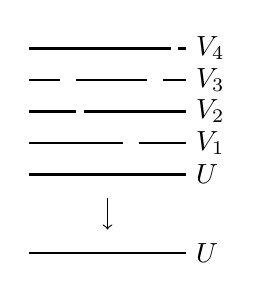
\begin{tikzpicture}
        \node (U) at (2, 0) [right] {\(U\)};
        \node (U') at (2, 1) [right] {\(U\)};
        \node (V1) at (2, 1.4) [right] {\(V_1\)};
        \node (V2) at (2, 1.8) [right] {\(V_2\)};
        \node (V3) at (2, 2.2) [right] {\(V_3\)};
        \node (V4) at (2, 2.6) [right] {\(V_4\)};
        \draw[thick] (0, 0) -- (2, 0);
        \draw[thick] (0, 1) -- (2, 1);
        \draw[thick] (0, 1.4) -- (1.2, 1.4); \draw[thick] (1.4, 1.4) -- (2, 1.4);
        \draw[thick] (0, 1.8) -- (0.6, 1.8); \draw[thick] (0.7, 1.8) -- (2, 1.8);
        \draw[thick] (0, 2.2) -- (0.4, 2.2); \draw[thick] (0.6, 2.2) -- (1.5, 2.2); \draw[thick] (1.7, 2.2) -- (2, 2.2);
        \draw[thick] (0, 2.6) -- (1.8, 2.6); \draw[thick] (1.9, 2.6) -- (2, 2.6);
        \draw[->] (1, .7) -- (1, .3);
    \end{tikzpicture}
    \caption{The presheaf $F = h_U$ represented by $U\subseteq X$ of \cref{exmp:representable-presheaf-espace-étalé}.}
    \label{fig:presheaf-represented-by-U}
\end{figure}

\begin{rmk}
In general, the étalé space $\etalespace(F)$ is not `computable'.
It is, however, when $F$ is \emph{constructible}\index{constructible sheaf}, which we will see in one of the final lectures.\todo{Ref back}
\end{rmk}

\begin{prop}
    The construction of the étalé space defines a functor
    $\catSheaf(X) \to \catTopologicalSpace_{/X}$.
\end{prop}
\begin{proof}
    We can cheat and use the unproven remark that the étalé space is a \indexterm{coend}. \todo{prove?}
\end{proof}

\subfile{Lectures/Lecture 3}
\chapter{Sheafification, monodromy}\label{lecture:4}

\section{Sheaf/space adjunction (continued)}
\remyquote{Computers don't have noses.}
\noindent
We still have to prove that the counit of the sheaf/space adjunction is an isomorphism for local homeomorphisms to prove the equivalence $\catSheaf(X)\simeq\catLocalHomeomorphism_{/X}$.

\begin{proof}[of the restricted equivalence in \cref{thm:sheaf-space-adjunction}, continued]
If $f\colon Y\to X$ is a local homeomorphism, we have to show that the counit
\[ \epsilon_{Y/X} \colon \etalespace(h_{Y/X}) \to Y \]
is an isomorphism in $\catLocalHomeomorphism_{/X}$ (or $\catTopologicalSpace_{/X}$).
Concretely, this map is given by
\begin{equation*}
    \begin{tikzcd}[column sep=small]
        \coprod_{U\subseteq X}\cont[X](U,Y)\times U \ar[rr] \ar[rd, epi] & & Y \\
        & \etalespace(h_{Y/X}) \ar[ru, "\epsilon_{Y/X}"']
    \end{tikzcd}
\end{equation*}
where the top map sends $(s,x)_U$ to $s(x)\in Y$.
This map indeed descends to the étalé space $\etalespace(h_{Y/X})$: if $x\in U\subseteq V$ and $s\colon V\to Y$ is a section, then $(s,x)_V\sim(s|_U,x)_U$, and both are sent to $s(x)$.

By \cref{lem:localhomtriangle,lem:etalelocalhomeo}, the map $\etalespace(h_{Y/X})\to Y$ is a local homeomorphism, so in particular an open map, so it suffices to check that it is bijective.

For injectivity, assume $\epsilon_{Y/X}([s,x]_U)=\epsilon_Y([t,y]_V)$.
Then $x=y$ since everything is over $X$, and thus \(s(x)=t(x)\) by assumption.
Let \(S\) be an open neighbourhood of \(s(x)=t(x)\) in \(Y\) such that \(f\) restricts to a homeomorphism \(f|_S\colon S\to f(S)\), and set \(W\coloneq s\inv(S)\cap t\inv(S)\).
Observe that \(W\) contains \(x\).
Then \(s|_W\) and \(t|_W\) are both sections to the injective map \(f|_S\colon S\hookrightarrow X\), so they agree.
Hence \((s,x)_U\approx(s|_W,x)_W=(t|_W,x)_W\approx(t,x)_V\) and we conclude that \(\epsilon_{Y/X}\) is injective.

For surjectivity, let \(y\in V\) and set \(x=f(y)\in X\).
Choose an open neighbourhood \(V\subseteq Y\) of \(y\) such that \(f\) restricts to a homeomorphism \(f|_V\colon V\to f(V) \eqcolon U\) onto an open subset.
Write \(s\colon U\to V\) for its inverse \(f|_V\inv\); then \(s\colon U\to V\subseteq Y\) is a section with \(s(x)=y\), so \(\epsilon_{Y/X}([s,x]_U)=y\), showing that \(\epsilon_{Y/X}\) is surjective.

We conclude that the counit of the sheaf/space adjunction is an isomorphism for local homeomorphisms, finishing the proof of the equivalence of categories \(\catSheaf(X)\simeq\catLocalHomeomorphism_{/X}\) of \cref{thm:sheaf-space-adjunction}.
\end{proof}

\begin{defn}
For a space $X$, the composite functor
\[ (-)^\sharp \coloneq h_{-/X} \circ \etalespace* \colon \catPresheaf(X)\to\catSheaf(X) \]
is called \indexdefnemph{sheafification}.
It comes with a natural map $F\To F^\sharp$ for presheaves $F$ on $X$ given by the unit of the adjunction $\etalespace*\leftadj h_{-/X}$.
\end{defn}

The following result can be seen as the universal property of sheafification\index{sheafification!universal property}.

\begin{cor}\label{cor:sheafification-left-adjoint-to-inclusion}
Sheafification is left adjoint to the inclusion $\catSheaf(X)\hookrightarrow\catPresheaf(X)$.
That is, if $F$ is a presheaf on $X$ and $\mathcal G$ is a sheaf on $X$, then every map $F\To \mathcal G$ of presheaves factors uniquely through the natural map $F\To F^\sharp$.
\end{cor}
\begin{proof}
Compose the adjunction $\etalespace*\leftadj h_{-/X}$ and the equivalence $\catLocalHomeomorphism_{/X}\simeq\catSheaf(X)$.
\end{proof}

The unit of the adjunction is the map $F\To F^\sharp$; it is an isomorphism if and only if $F$ is a sheaf.

\begin{exmp}\label{exmp:sheaf-on-point-set}
For the one-point space $*$, we have $\open(*) = \{\emptyset\hookrightarrow *\}$, so
\[ \catPresheaf(X) = \catFunctor(\mathord{\to},\catSet) \]
is the arrow category of $\catSet$.
As we have seen in the homework, a presheaf $F$ on the one-point space -- that is, a map $F(*)\to F(\emptyset)$ -- is a sheaf if and only if $F(\emptyset)=*$.
Hence we have an equivalence $\catSheaf(X)\simeq\catSet$.
Of course, we also have $\catLocalHomeomorphism_{/*} \simeq\catSet$ since having a local homeomorphism $X\to *$ implies $X$ is discrete.
\end{exmp}

\begin{exmp}
Let $S=\{0,1\}$ be the \indexterm{Sierpiński space} with
\[ \open(S) = \{\emptyset\hookrightarrow\{1\}\hookrightarrow S\}\text{.} \]
Using a similar argument as in the previous example, we see
\[ \catPresheaf(S) \simeq \catFunctor(\mathord{\to}\mathord{\to},\catSet) \]
and
\[ \catSheaf(S) \simeq \catFunctor(\mathord{\to},\catSet)\text{.} \]
\end{exmp}

\begin{exc}
Check that sheafification on $S$ is given by sending a presheaf $F$ -- that is, a pair of maps $F(S)\to F(\{1\})\to F(\emptyset)$ -- to the sheaf given by the map $F(S)\to F(\{1\})$.
\end{exc}

\section{Restriction of sheaves}
\remyquote{You can do this for different values of four, here we do it for five.}

\begin{defn}
Let $U\subseteq X$ be open and let $F$ be a presheaf on $X$.
Then the \emph{restriction}\index{restriction!of sheaves} $F|_U$ of $F$ to $U$ is the restriction of the functor $F$ along the inclusion $\open(U)\hookrightarrow\open(X)$.
\end{defn}

\begin{lem}
If $\mathcal F$ is a sheaf on $X$, then so is its restriction $\mathcal F|_U$ to an open $U\subseteq X$.
Under the equivalence $\catSheaf(X)\simeq\catLocalHomeomorphism_{/X}$, restriction to $U$ corresponds to sending a local homeomorphism $f\colon Y\to X$ to the \indexterm{pullback} $f\inv(U)\to U$.
\end{lem}

In $\catLocalHomeomorphism_{/X}$, we have the subcategory $\catCoveringSpace_{/X}$ of \emph{covering spaces}\index{covering space}: continuous maps $f\colon Y\to X$ such that $X$ has an open cover $X = \bigcup_{i\in I}U_i$ and there are sets $S_i$ such that $f\inv(U_i)\to U_i$ is isomorphic to $U_i\times S_I\to U_i$ (where $S_i$ has the discrete topology) over $U_i$ for all $i\in I$.

\todo{Pancake example}

\begin{rmk}
We will not assume that the space $Y$ in a covering space $Y\to X$ is (path) connected; this condition does appear in the literature with some authors.
\end{rmk}

\begin{defn}
A sheaf $\mathcal F$ on a space $X$ is \emph{locally constant}\index{sheaf!locally constant} if there is an open cover $X = \bigcup_{i\in I}U_i$ such that the restriction $\mathcal F|_{U_i}$ is a constant sheaf $h_{S_i}$ for some set $S_i$ for all $i\in I$.

We write $\catLocallyConstantSheaf(X)$ for the full subcategory of $\catSheaf(X)$ on the locally constant sheaves.
\end{defn}

\begin{lem}
Under the equivalence $\catSheaf(X)\simeq\catLocalHomeomorphism_{/X}$, the locally constant sheaves correspond to covering spaces.
In other words, this equivalence restricts to an equivalence
\[ \catLocallyConstantSheaf(X) \simeq \catCoveringSpace_{/X}\text{.} \]
\end{lem}

The real content is the constant case: we have $\mathcal F\cong h_S = h_{X\times X/X}$ if and only if $\etalespace(\mathcal F)\cong X\times S$ over $X$.
% \begin{proof}
% First, let $\mathcal F$ be a locally constant sheaf on $X$.
% Then there is an open cover $X = \bigcup_{i\in I}U_i$ such that $\mathcal F|_{U_i}\cong h_{S_i}$ for some set $S_i$ for all $i\in I$.
% \end{proof}

\todo{Four-to-one cover of the circle example}

\section{Review of monodromy}
\remyquote{If you've ever been in a parking garage, you know what I mean.}

\begin{figure}[h!]
  \centering
  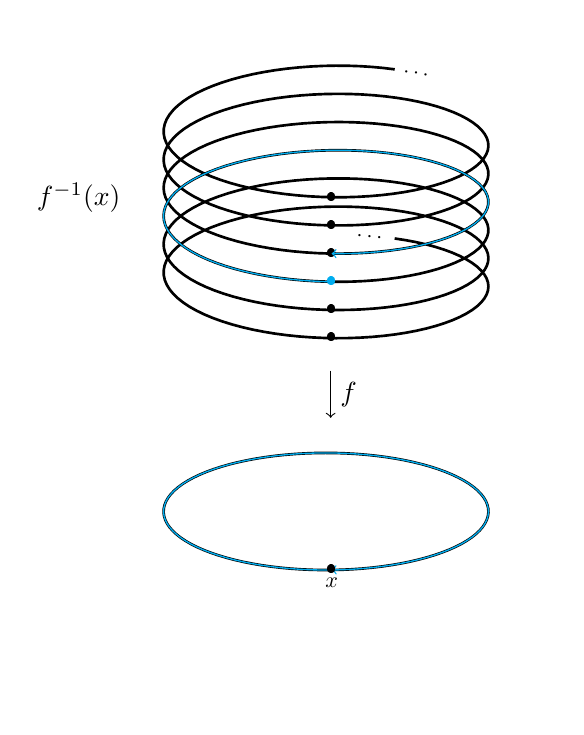
\begin{tikzpicture}[scale=.8]
    \begin{axis}[axis line style={draw=none}, tick style={draw=none}, xticklabel=\empty, yticklabel=\empty, zticklabel=\empty]
      \addplot3+[domain=0:12*pi,samples=500,samples y=0,black,no marks,very thick]
        ({sin(deg(x))}, {cos(deg(x))}, {6*x/(pi)})
        node[pos=0, left, rotate=-5] {\ldots}
        node[pos=1, right, rotate=-10] {\ldots}
        node[pos=0.85/12] {\textbullet}
        node[pos=2.85/12] {\textbullet}
        node[pos=6.85/12] {\textbullet}
        node[pos=8.85/12] {\textbullet}
        node[pos=10.85/12] {\textbullet};
      \addplot3+[domain=4.85*pi:6.85*pi,samples=500,samples y=0,cyan,no marks,semithick,->] ({sin(deg(x))}, {cos(deg(x))}, {6*x/(pi)}) node[pos=0] {\textbullet};
    \end{axis}
    \node at (-0.5,3) {\(f^{-1}(x)\)};
    \draw[->] (3.5,.25) -- (3.5,-0.5) node[right] at (3.5,-0.125) {\(f\)};
    \begin{axis}[axis line style={draw=none}, tick style={draw=none}, xticklabel=\empty, yticklabel=\empty, zticklabel=\empty, at={(0,0,-300)}]
      \addplot3+[domain=0.85*pi:2.85*pi,samples=100,samples y=0,black,no marks,very thick]
        ({sin(deg(x))}, {cos(deg(x))}, {0});
      \addplot3+[domain=0.85*pi:2.85*pi,samples=100,samples y=0,cyan,no marks,semithick,->]
        ({sin(deg(x))}, {cos(deg(x))}, {0})
        node[pos=0,black] {\textbullet}
        node[pos=0,black,below] {\(x\)};
    \end{axis}
  \end{tikzpicture}
  \caption{Unique path lifting in the cover of the circle by the helix}
  \label{fig:unique-path-lifting-circle-helix}
\end{figure}

\begin{defn}
    Let $X$ be a topological space. Then $X$ is 
    \begin{enumerate}
        \item \emph{locally path connected} if every open neighbourhood $x \in U$ of any $x \in X$ contains a path connected open neighbourhood $x \in V \in U$.
        \item \emph{semi-locally path connected} if for every $x \in X$, there exists an open neighbourhood $x\in U$ such that the map $\homotopy[1](U, x) \to \homotopy[1](X,x)$ is trivial. 
    \end{enumerate}
\end{defn}

\begin{defn}
    Let $X$ be a topological space and $x\in X$. The \indexdefnemph{fibre functor} is defined by
    \begin{align*}
        F_x: \catCoveringSpace_{/X} &\to \homotopy[1](X,x)\catSet\\
        (Y \xrightarrow{f} X) &\mapsto f^{-1}(x),
    \end{align*}
    where a loop $\gamma \in \homotopy[1](X,x)$ acts on $f^{-1}(x)$ by unique path lifting. 
\end{defn}

\begin{thm}[name={\indexterm{monodromy} correspondence}]
    Let $X$ be a topological space and $x \in X$. 
    \begin{enumerate}
        \item If $X$ is path connected and locally path connected, then
        \[
            F_x: \catCoveringSpace_{/X} \to \homotopy[1](X,x)\catSet
        \] is fully faithful. 
        \item If $X$ is moreover semi-locally simply connected, then $F_x$ is an equivalence of categories. 
    \end{enumerate}
\end{thm}
\begin{proof}[outline]\todo{Maybe type up the details Marcel}
    \begin{itemize}
        \item Any covering $f: Y \to X$ is locally path connected (easy). It is furthermore a disjoint union $\coprod_{i \in I} Y_i$ of path connected spaces $Y_i$ \cite[Theorem~25.4]{MunkresTopology}.
        \item Any map $Y \xrightarrow{\phi}Y' \in \catCoveringSpace_{/X}$ is itself a covering \cite[Lemma~80.2(a)]{MunkresTopology}.
        \item $F_x$ is faithful: if two maps 
        \[
            \begin{tikzcd}
                Y \arrow[rr, "\phi'"', shift right] \arrow[rr, "\phi", shift left] \arrow[rd, "f"'] &   & Y \arrow[ld, "f'"] \\
                & X & 
            \end{tikzcd}
        \] agree on $f^{-1}(x)$ then they agree: for $y \in Y$ arbitrary, choose a path $\gamma$ starting at $f(y)$ and ending at $x$. By unique path lifting, this gives a path $\overline{\gamma}$ from $y$ to $y'$ for some $y' \in f^{-1}(x)$. Then $\phi(\overline{\gamma})$ and $\phi'(\overline{\gamma})$ are both lifts of $\gamma$ to paths ending at $\phi'(y') = \phi(y')$ so by uniqueness they are the same path and their starting points are the same, i.e. $\phi(y) = \phi'(y)$. 
        \item That $F_x$ is full follows from the lifting lemma \cite[Lemma~79.1]{MunkresTopology}.
        \item $F_x$ is essentially surjective if $X$ is semi-locally simply connected: every $S \in \homotopy[1](X,x)\catSet$ is $S \cong \cup_{i\in I}S_i$ where $\homotopy[1](X,x)$ acts transitively on $S_i$. \todo{explain} Then \[
            S_i \cong \homotopy[1](X,x) / H_i
        \] for $H_i = \text{Stab}(s_i)$ for any $s_i \in S_i$. There exists a covering $Y_i \xrightarrow{f_i} X$ with $\homotopy[1](Y_i, y_i) \xhookrightarrow{} \homotopy[1](X,x)$, one subgroup $H_i$ \cite[Theorem~82.1]{MunkresTopology}, so $S_i \cong F_x(Y_i \xrightarrow{f_i} X)$ and $S = F_x(\coprod_{i \in I} Y_i \to X)$.
        \end{itemize}
\end{proof}
\begin{exmp}
Let $X = S^1$. Let $Y_1$ be the four-to-one covering of $S^1$, and let $Y_2$ be the double covering of $S^1$. Let $Y = Y_1 \coprod Y_2$. Then $Y \to X$ corresponds to the set $\{1,2,3,4,5,6\}$ where the single loop around the circle $1\in \homotopy[1](S^1, x)$ acts by $(12)(3456)$ \todo{Diagram below should have labels etc}.
\begin{figure}
\centering
% https://tex.stackexchange.com/a/495715
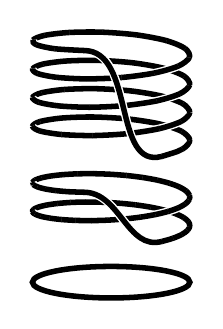
\begin{tikzpicture}[declare function={f(\x)=0.2*sin(\x)+\x/1000;},
 rubout/.style={/utils/exec=\tikzset{rubout/.cd,#1},
 decoration={show path construction,
      curveto code={
       \draw [white,line width=\pgfkeysvalueof{/tikz/rubout/line width}+2*\pgfkeysvalueof{/tikz/rubout/halo}] 
        (\tikzinputsegmentfirst) .. controls
        (\tikzinputsegmentsupporta) and (\tikzinputsegmentsupportb)  ..(\tikzinputsegmentlast); 
       \draw [line width=\pgfkeysvalueof{/tikz/rubout/line width},shorten <=-0.1pt,shorten >=-0.1pt] (\tikzinputsegmentfirst) .. controls
        (\tikzinputsegmentsupporta) and (\tikzinputsegmentsupportb) ..(\tikzinputsegmentlast);  
      }}},rubout/.cd,line width/.initial=2pt,halo/.initial=0.5pt]
 \draw[rubout={line width=2pt,halo=0.5pt},decorate] 
   plot[variable=\x,domain=-50:1330,samples=55,smooth] ({cos(\x)},{f(\x)}) to[out=0,in=195] cycle;
 \draw[rubout={line width=2pt,halo=0.5pt},decorate] 
   plot[variable=\x,domain=-1130:-470,samples=55,smooth] ({cos(\x)},{f(\x)}) to[out=0,in=195] cycle;

 \draw[line width=2pt] (0,-2) arc(-90:270:1cm and 0.2cm);
 % \draw[thick,-stealth]  (0,-0.4) -- (0,-1.4) node[midway,right]{$p$};
\end{tikzpicture}
\caption{Covering of the circle by a disjoint union of the four-to-one cover and the two-to-one cover.}
\label{fig:circle-cover-quadruple-double}
\end{figure}
\end{exmp}

The following diagram summarises the situation if $X$ is a `nice' space:
\begin{equation*}
    \begin{tikzcd}
        \catSheaf(X) \ar[r, "\simeq"] & \catLocalHomeomorphism_{/X} \\
        \catLocallyConstantSheaf(X) \ar[u, inclusion] \ar[r, "\simeq"'] & \catCoveringSpace_{/X} \ar[u, inclusion] \ar[r, "\simeq"'] & \homotopy[1](X,x)\catSet
    \end{tikzcd}
\end{equation*}
This diagram raises the question: what should there be in the top right spot?
Towards the end of the course, we will give a partial answer which goes by the name of \indexemph{exodromy}.

\chapter{Pullback and pushforward}

\remyquote{There is a risk you might learn something -- beware!}
\noindent
The goal of this lecture is to define a pair of adjoint functors
\begin{equation*}
  \begin{tikzcd}
    \catSheaf(Y) \ar[r, "f_*"'{name=rightadj}, shift right=2] &
    \catSheaf(X) \ar[l, "f^*"'{name=leftadj}, shift right=2]
    \ar[from=leftadj, to=rightadj, phantom, "\leftadj" rotate=-90]
  \end{tikzcd}
\end{equation*}
for a continuous map \(f\colon Y\to X\), called \indexemph{pullback} and \indexemph{pushforward}.
The strategy will be to first define these operations for presheaves, and then restrict to sheaves.
One of the functors will already send sheaves to sheaves, for the other we will postcompose the functor on the level of presheaves with sheafification.

\section{Pushforward}

A continuous map \(f\colon Y\to X\) induces a functor \(f\inv\colon\open(X)\to\open(Y)\) which sends an open set \(U\subseteq X\) to the open set \(f\inv(U)\subseteq Y\).
If \(U\subseteq V\subseteq X\) are open sets, then \(f\inv(U)\subseteq f\inv(V)\subseteq Y\), so this is indeed functorial.

\begin{defn}
The \indexdefnemph{pushforward} of a presheaf \(G\) on \(Y\) along \(f\) is the composite presheaf
\begin{equation*}
  f_*G \colon \open(X)\opp \xrightarrow{f\inv} \open(Y)\opp \xrightarrow{G} \catSet
\end{equation*}
on \(X\).
Explicitly, the value of the pushforward \(f_*G\) on an open \(U\subseteq X\) is \((f_*G)(U) = G(f\inv(U))\).
\end{defn}

The pushforward functor \(f_*\colon\catPresheaf(Y)\to\catPresheaf(X)\) is given by precomposition by the functor \(f\inv\colon\open(X)\opp\to\open(Y)\opp\), and so is indeed seen to be functorial.

\begin{lem}
If \(\mathcal G\) is a sheaf on \(Y\), then the pushforward \(f_*\mathcal G\) of \(\mathcal G\) along \(f\) is a sheaf on \(X\).
In particular, pushforward restricts to a functor \(f_*\colon\catSheaf(Y)\to\catSheaf(X)\) on the level of sheaves.
\end{lem}
\begin{proof}
Let \(U=\bigcup_{i\in I}U_i\) be an open cover in \(X\).
Then \(f\inv(U) = \bigcup_{i\in I}f\inv(U_i)\) is an open cover in \(Y\).
Applied to this cover, the sheaf condition for \(\mathcal G\) gives us an equaliser diagram
\begin{equation*}
  \begin{tikzcd}
    \mathcal G(f\inv(U)) \ar[r] & \prod_{i\in I}\mathcal G(f\inv(U_i)) \ar[r, shift left] \ar[r, shift right] & \prod_{i,j\in I}\mathcal G(f\inv(U_i\cap U_j))
  \end{tikzcd}
\end{equation*}
(where we have rewritten \(f\inv(U_i)\cap f\inv(U_j)=f\inv(U_i\cap U_j)\)), giving the sheaf condition for the pushforward \(f_*\mathcal G\).
\end{proof}

\section{Pullback}
\remyquote{Just sheafify the hell out of everything.}
\noindent
The \indexemph{pullback} of a sheaf on \(X\) along \(f\) should be a sheaf on \(Y\).
One way to approach the problem of constructing a presheaf on \(Y\) from a presheaf \(\mathcal F\) on \(X\), would be to try extending it along \(f\inv\) (and this is what we will attempt):
\begin{equation*}
  \begin{tikzcd}[column sep=tiny]
    \open(X)\opp \ar[rr, "\mathcal F"] \ar[rd, "f\inv"'] & & \catSet \\
    & \open(Y)\opp \ar[ru, dashed, "?"']
  \end{tikzcd}
\end{equation*}
In general, there might not be such an on-the-nose extension, but we can approximate an extension by considering extensions \emph{up to} a natural transformation.
There could be many such approximations, so we want to consider the `best possible approximation' in some suitable sense.

In category theory, the general problem of approximating an extension of a functor along another functor is studied using \indexemph{Kan extensions}; we refer to~\cite[Chapter~6]{riehlCategoryTheoryContext2016} for an introduction of Kan extensions, whose definition we actually do not need to know for our current purposes.
Here we will apply the general theory to our case to define the pullback of sheaves.\footnote{One can also construct and prove everything by hand, as was done in class, but this is rather tedious. We wish to illustrate with the following exposition that all the arguments will be completely formal.}

\begin{prop}\label{prop:pullback-Kan-extension}
Left Kan extensions\index{Kan extension} of presheaves on \(X\) (functors \(\open(X)\opp\to\catSet\)) along the functor \(f\inv\colon\open(X)\opp\to\open(Y)\opp\) exist, and assemble into a functor
\[\Lan*_{f\inv}\colon\catPresheaf(X)\to\catPresheaf(Y)\]
which is left adjoint to the \indexterm{pushforward} functor \(f_*\):
\begin{equation*}
  \begin{tikzcd}
    \catPresheaf(Y) \ar[r, "f_*"'{name=rightadj}, shift right=2] &
    \catPresheaf(X) \ar[l, "\Lan*_{f\inv}"'{name=leftadj}, shift right=2]
    \ar[from=leftadj, to=rightadj, phantom, "\leftadj" rotate=-90]
  \end{tikzcd}
\end{equation*}
Moreover, the left Kan extension along \(f\inv\) of a presheaf \(F\) on \(X\) is given on opens \(U\subseteq Y\) by
\begin{equation} \label{eq:left-Kan-extension-f-inv-colimit}
  \Lan_{f\inv} F(U) = \colim\displaylimits_{f\inv(W)\supseteq U}F(W)
\end{equation}
where \(W\) ranges over opens of \(X\) (more precisely, the colimit diagram is indexed by the full subcategory of \(\open(X)\) on those \(W\) such that \(f\inv(W)\supseteq U\), or equivalently \(W\supseteq f(U)\)).
\end{prop}
\begin{proof}
This is a special case of~\cite[Corollary~6.2.6]{riehlCategoryTheoryContext2016}; the only nontrivial step in applying the general result to this special case is recognising that the comma category \(f\inv\downarrow U\) for \(U\in\open(Y)\opp\) is the described index category, but this verification is elementary enough to be left to the reader.
\end{proof}

We would also like a description of what \(\Lan*_{f\inv}\) does on maps.
By a computation of the colimit in \cref{eq:left-Kan-extension-f-inv-colimit}, an element of \(\Lan*_{f\inv} F(U)\) is given by \([s]_W\) for some section \({s\in F(W)}\) for some \(W\supseteq f(U)\), where \([s]_W = [s']_{W'}\) if and only if there exists an open \(W''\subseteq W\cap W'\) containing \(f(U)\) such that \(s|_{W''} = s'|_{W''}\).
Unravelling the construction in \cite[Theorem~6.2.1]{riehlCategoryTheoryContext2016}, we see that the map induced by opens \(U\subseteq V\) in \(Y\) is given by
\[ \colim\displaylimits_{f\inv(W)\supseteq V}F(W) \to \colim\displaylimits_{f\inv(W)\supseteq U}F(W)\text{,} \quad [s]_W \mapsto [s]_W\text{.} \]

We may now define the pullback as follows:
\begin{defn}
The \emph{pullback}\index{pullback!of presheaves} \(f^{\circledast}F\) of a presheaf \(F\) on \(X\) along \(f\) is the left Kan extension of \(F\) along \(f\inv\).
The pullback functor is denoted \(f^{\circledast}\coloneq\Lan*_{f\inv}\colon\catPresheaf(X)\to\catPresheaf(Y)\).
\end{defn}

We have defined the pullback functor in such a way that it is left adjoint to the pushforward of presheaves.

We use the circled asterisk \(\circledast\) in the notation for the pullback of presheaves to distinguish it from the pullback of sheaves, which we will define momentarily, and for which we use a normal asterisk.\footnote{In class, we used the notation $f^{\textup{pre,*}}$ for $f^\circledast$, which we do not find very elegant.}
Unlike the pushforward, namely, the pullback of presheaves does not directly restrict to sheaves; that is to say, there are sheaves which are sent by \(f^{\circledast}\) to a presheaf which does not satisfy the sheaf condition, as witnessed by the following counterexample:

\begin{exmp}
Let $Y$ be the two-point space with the discrete topology, and let $X$ be the one-point space, with the unique map $f: Y \to X$. 
We can easily put a sheaf on $X$, for example by defining $\mathcal{F}(\emptyset) = *$ and $\mathcal{F}(X) = \{42, 43, 44\}$. 
The pullback in presheaves at any point $\{*\} \subset Y$ is $f^{\circledast}(\{*\}) = \colim_{f^{-1}(W) \supseteq *}\mathcal{F}(W) = \mathcal{F}(X) = \{42, 43, 44\}$. But the pullback in presheaves at $Y$ itself is also $\mathcal{F}(X) = \{42, 43, 44\}$. Check that the sheaf condition doesn't hold for the cover of $Y$ given by two opens, one containing precisely each point: the gluing condition on $\{42,43,44\} \times \{42, 43, 44\}$ is void because the points do not intersect.
\end{exmp}

\begin{defn}
The \emph{pullback}\index{pullback!of sheaves} \(f^*\mathcal F\) of a sheaf \(\mathcal F\) on \(X\) along a continuous map \(f\colon Y\to X\) is the sheaf
\[ f^*\mathcal F \coloneq (f^{\circledast}\mathcal F)^\sharp \]
on \(Y\), the sheafification of the presheaf pullback of \(\mathcal F\).
The pullback functor of sheaves is thus the composite
\[ f^* \colon \catSheaf(X) \hookrightarrow \catPresheaf(X) \xrightarrow{f^{\circledast}} \catPresheaf(Y) \xrightarrow{(-)^\sharp} \catSheaf(Y)\text{.} \]
\end{defn}

Note that the definition of the pullback also makes sense for presheaves; we also denote the functor \(\catPresheaf(X)\to\catSheaf(Y)\) sending a presheaf \(F\) to the pullback \(f^*F = (f^\circledast)^\sharp\) by \(f^*\).

\begin{prop}\label{lem:pushforward-pullback-adjunction-sheaves}
Pushforward and pullback of sheaves along \(f\) define an adjunction
\begin{equation*}
  \begin{tikzcd}
    \catSheaf(Y) \ar[r, "f_*"'{name=rightadj}, shift right=2] &
    \catSheaf(X) \ar[l, "f^*"'{name=leftadj}, shift right=2]
    \ar[from=leftadj, to=rightadj, phantom, "\leftadj" rotate=-90]
  \end{tikzcd}
\end{equation*}
\end{prop}
\begin{proof}
Compose the adjunctions
\begin{equation*}
  \begin{tikzcd}
    \catSheaf(Y) \ar[r, ""'{name=rightadj1}, inclusion, shift right=2] \ar[rrd, "f_*"', bend right=15] &
    \catPresheaf(Y) \ar[l, "(-)^\sharp"'{name=leftadj1}, shift right=2] \ar[r, "f_*"'{name=rightadj2}, shift right=2] &
    \catPresheaf(X) \ar[l, "f^{\circledast}"'{name=leftadj2}, shift right=2] \ar[ll, "f^*"', bend right=15, shift right=5] \\
    & & \catSheaf(X) \ar[u, inclusion]
    \ar[from=leftadj1, to=rightadj1, phantom, "\leftadj" rotate=-90]
    \ar[from=leftadj2, to=rightadj2, phantom, "\leftadj" rotate=-90]
  \end{tikzcd}
\end{equation*}
of \cref{cor:sheafification-left-adjoint-to-inclusion} and \cref{prop:pullback-Kan-extension}.
\end{proof}

Between the sets $\Hom[\catSheaf(Y)](f^*\mathcal F,\mathcal G)$ and $\Hom[\catSheaf(X)](\mathcal F,f_*\mathcal G)$ which are naturally isomorphic by the adjunction, there is also an `intermediate' set of maps, called \emph{$f$-maps}; see~\cite[\href{https://stacks.math.columbia.edu/tag/008K}{Lemma 008K}]{stacks-project}.

From the fact that the pushforward already sends sheaves to sheaves (so its definition `doesn't need sheafification'), we obtain the following corollary, showing that pulling back the sheafification of a presheaf is the same as pulling back the presheaf.

\begin{cor}\label{cor:pullback-sheafification}
Let \(f\colon Y\hookrightarrow X\) be a continuous map.
Then the functors
\[ \catPresheaf(X) \xrightarrow{f^*} \catSheaf(Y) \qquad \text{and} \qquad \catPresheaf(X) \xrightarrow{(-)^\sharp} \catSheaf(X) \xrightarrow{f^*} \catSheaf(Y) \]
are naturally isomorphic.
\end{cor}
\begin{proof}
  % and write \(\iota\colon\catSheaf(X)\hookrightarrow\catPresheaf(X)\) for the full subcategory inclusion
By definition, the former functor is the composite
\begin{equation*}
  \begin{tikzcd}
    \catPresheaf(X) \ar[r, "f^\circledast"{name=leftadj1}, shift left=2] &
    \catPresheaf(*) \ar[l, "f_*"{name=rightadj1}, shift left=2] \ar[r, "(-)^\sharp"{name=leftadj2}, shift left=2] &
    \catSheaf(*) \ar[l, ""{name=rightadj2}, shift left=2, inclusion]
    \ar[from=leftadj1, to=rightadj1, phantom, "\leftadj" rotate=-90]
    \ar[from=leftadj2, to=rightadj2, phantom, "\leftadj" rotate=-90]
  \end{tikzcd}
\end{equation*}
of the presheaf pullback along \(f\) and sheafification, which have right adjoints given by respectively the pushforward along \(f\) and the full subcategory inclusion by \cref{prop:pullback-Kan-extension} and \cref{cor:sheafification-left-adjoint-to-inclusion}.
The latter functor has a right adjoint
\begin{equation*}
  \begin{tikzcd}
    \catPresheaf(X) \ar[r, "(-)^\sharp"{name=leftadj1}, shift left=2] &
    \catSheaf(X) \ar[l, ""{name=rightadj1}, shift left=2, inclusion] \ar[r, "f^*"{name=leftadj2}, shift left=2] &
    \catSheaf(*) \ar[l, "f_*"{name=rightadj2}, shift left=2]
    \ar[from=leftadj1, to=rightadj1, phantom, "\leftadj" rotate=-90]
    \ar[from=leftadj2, to=rightadj2, phantom, "\leftadj" rotate=-90]
  \end{tikzcd}
\end{equation*}
given by pushforward along \(f\) followed by the full subcategory inclusion by \cref{cor:sheafification-left-adjoint-to-inclusion} and \cref{lem:pushforward-pullback-adjunction-sheaves}.
These two right adjoint are equal by definition, so we find the required natural isomorphism.
\end{proof}

The following corollary roughly says that pushforward and pullback are `functorial in the map' (respectively co- and contravariantly).\footnote{This statement can probably be made precise in terms of \(2\)-categories.}

\begin{cor}
For any space \(X\), we have \((\id_X)_*=\id_{\catSheaf(X)}\cong(\id_X)^*\), and for any maps \(f\colon Z\to Y\) and \(g\colon Y\to X\) we have \((gf)_*=g_*f_*\colon\catSheaf(Z)\to\catSheaf(X)\) and \((gf)^*\cong f^*g^*\colon\catSheaf(X)\to\catSheaf(Z)\).
\end{cor}
Note that the identities for the pushforward hold on-the-nose, whereas we only prove the identities for the pullback up to natural isomorphism.
\begin{proof}
The identities for the pushforward follow directly from the definition since \((gf)\inv(U)=f\inv(g\inv(U))\).
The identities for the pullback follow from those for the pushforward and the adjunction of \cref{lem:pushforward-pullback-adjunction-sheaves}: we have adjunctions \((gf)^*\leftadj(gf)_*\) and \(f^*g^*\leftadj g_*f_*\) and the right adjoints in these adjunctions are equal.
\end{proof}

\section{Stalks, germs, skyscrapers}

\begin{defn}\label{defn:stalk}
Let $i_x\colon \{x\} \hookrightarrow X$ be the inclusion of a point in a space.
Then $i_x^* \mathcal{F}$ is the \indexdefnemph{stalk} $\mathcal{F}_x$ of $\mathcal{F}$ at $x$; this is a sheaf on a point, so equivalently a set by \cref{exmp:sheaf-on-point-set} (the value of the sheaf on the whole space).
Unravelling definitions, we have \[
    \mathcal{F}_x = \colim_{U \ni x} \mathcal{F}(U)\text{.}
\]
An element of the stalk at $x$ is represented by a \indexdefnemph{germ} $[s]_U$ for $U \ni x$ and $s \in \mathcal{F}(U)$, where \([s]_U = [t]_V\) if and only if there exists an open neighbourhood \(W\subseteq U\cap V\) of \(x\) such that \(s|_W=t|_W\).
\end{defn}
Note that the stalk $\mathcal{F}_x$ is the fibre of $\etalespace(X) \to X$ over $x$. 

\begin{rmk}
\Cref{cor:pullback-sheafification} tells us that we can compute the stalks of the sheafification of a presheaf by computing the stalks of the presheaf itself.
\end{rmk}

\begin{exmp}[orientation sheaf of a \indexterm{manifold}]
Let \(M\) be an \(n\)-dimensional topological manifold, by which we mean a Hausdorff space that is locally homeomorphic to \(\bb R^n\) (i.e., every point of \(M\) admits a neighbourhood homeomorphic to \(\bb R^n\)).
For a subset \(K\subseteq M\), we write \[H_k(M\mid K;R) \coloneq H_k(M,M\setminus K;R)\] for the \(k\)th homology of \(M\) relative to \(M\setminus K\) with coefficients in a commutative ring \(R\).

A \emph{local \(R\)-orientation} at a point \(x\in M\) is a generator \(\mu_x\) of \(H_n(M\mid x;R)\cong R\) (note that we take homology in degree \(n\), the dimension of the manifold \(M\)).
That \(H_n(M\mid x;R)\) is isomorphic to \(R\) (as \(R\)-modules) follows from excision; choosing a generator corresponds exactly to choosing such an isomorphism.
An \emph{\(R\)-orientation}\index{manifold!orientation} of \(M\) is a family of local orientations \((\mu_x)_{x\in M}\) with the property that every point \(y\in M\) admits a compact neighbourhood \(K\) and an element \(\mu_K\in H_n(M\mid K;R)\) such that \(\mu_K\) restricts to \(\mu_x\) for any \(x\in K\) under the map \(H_n(M\mid K;R)\to H_n(M\mid x;R)\) induced by the inclusion \(M\setminus K\to M\setminus\{x\}\).

There is a sheaf \(\mathcal O_M\) of \(R\)-modules, the \emph{orientation sheaf}\index{manifold!orientation sheaf} of \(M\), defined by
\[\mathcal O_M(U)\coloneq H_n(M\mid U;R)\]
for \(U\subseteq M\) open.
The restriction map for opens \(U\subseteq V\subseteq M\) is induced by the inclusion of pairs \((M,M\setminus V)\hookrightarrow(M,M\setminus U)\).
The stalk of the orientation sheaf \(\mathcal O_M\) at \(x\in M\) is the \(R\)-module \(H_n(M\mid x;R)\).
\end{exmp}

\begin{rmk}
One can show (as a generalisation of an exercise in Homework 3) that the étalé space of the pullback can be obtained as a \indexterm{fibre product}. More precisely, given $f\colon Y \to X$, the diagram 
\[\begin{tikzcd}
	{\etalespace(f^*\mathcal{F})} & {\etalespace(\mathcal{F})} \\
	Y & X
	\arrow[from=1-1, to=2-1]
	\arrow[from=2-1, to=2-2]
	\arrow[from=1-2, to=2-2]
	\arrow[from=1-1, to=1-2]
	\arrow[pullback, from=1-1, to=2-2]
\end{tikzcd}\]
is a pullback square. 
This is used in \todo{Add cite MacLane Moerdijk} to define $f^*$. 
\end{rmk}


Given a map $\alpha\colon \mathcal{F} \to \mathcal{G}$ between sheaves on a space $X$ and a point $x \in X$, there is an induced map on stalks $\alpha_x\colon \mathcal{F}_x \to \mathcal{G}_x$, because $\mathcal{G}_x$ is a cocone over
\[\setpred{\mathcal{F}(U)}{U \in \open(X),x \in U}\text{,}\]
of which $\mathcal{F}_x$ is a colimit. 

\begin{lem}\label{lem:stalkwise-check-isomorphism}
    Let $\alpha\colon \mathcal{F} \to \mathcal{G}$ be a map in $\catSheaf(X)$. 
    Then $\alpha$ is an isomorphism of sheaves if and only if $\alpha_x\colon \mathcal{F}_x \to \mathcal{G}_x$ is a bijection for all $x \in X$. 
\end{lem}
\begin{proof}
    The map $\etalespace(\alpha)\colon \etalespace(\mathcal{F}) \to \etalespace(\mathcal{G})$ is a local homeomorphism over $X$, because the maps $\etalespace(\mathcal{F}) \to X$ and $\etalespace(\mathcal{G}) \to X$ are local homeomorphisms. In particular, $\etalespace(\alpha)$ is an open map. So it is invertible if and only if it is a bijection. Check that this is equivalent to requiring that the map on the fibres over $x$ is a bijection for all $x \in X$. Since the stalks $\mathcal{F}_x$ and $\mathcal{G}_x$ are exactly these fibres, we are done. 
\end{proof}

\begin{defn}
    Let $\{x\} \to X$ be the inclusion of a point $x \in X$. Let $S \in \catSet$. The \indexemph{skyscraper sheaf} at $x$ with value $S$ is $i_{x,*}\underline{S}$, the pushforward of the constant sheaf. We denote it $i_{*, S}$.
\end{defn}

\begin{exmp}
    Let $\{0\} \to \bb R$ be the inclusion of zero into the real numbers. Let $S = \{a,b\}$. Then the skyscraper sheaf is 
    \[
        i_{*,S}(U) = S(U \cap 0) =     \begin{cases}
        \{a,b\} & \text{if } 0 \in U\\
        * & \text{if } x \notin U.
    \end{cases}
    \]
    In Homework 2, we saw that the étalé space of this sheaf is the line with two origins. 
\end{exmp}
\subfile{Lectures/Lecture 6}
\subfile{Lectures/Lecture 7}
\subfile{Lectures/Lecture 8}
\printbibliography
\printindex

\end{document}
